\chapter{SCION Host Architecture}
\index{host architecture}

\section{Current host architecture} \chris{this describes the current status and is updated with our progress.}

Figure~\ref{fig:host} provides a high level overview of the SCION host architecture. The components are the following:

\begin{itemize}
\item \textit{Socket}
\index{socket}
In the current setting, the legacy socket code is used. The goal is to provide a SCION socket (AF\_SCION) that takes advantage
of the multiple SCION paths. 

\item \textit{TUN/TAP Interface} is used to enable packet processing in userspace. When applications send data,
the interface captures packets for specific destinations (for which communication proceeds over SCION). To capture
this traffic, routing entries that forward traffic to this interface are inserted in the main routing table. For
incoming traffic from the SCION network, the TUN/TAP interface is used to (re)inject the traffic in the
TCP/IP stack.

\item \textit{Interface between socket and scion\_path}
The details of this interface have to be determined. 
Currently, scion\_path operates as a gateway by encapsulating/decapsulating the SCION header.
The purpose is to give more control to the TCP stack in order to implement a MP-TCP with
higher control levels.


\item \textit{Scion\_path}
The scion\_path daemon runs in userspace and has collected SCION paths (the corresponding OFs) for destination ADs.
For outgoing packets, the daemon inserts the corresponding OFs in a SCION header and then forwards the traffic
to the next SCION node on the path (a SCION border router). For incoming traffic from SCION, the daemon strips
the SCION header and writes the remaining data to the TUN/TAP interface. The interface considers this data as incoming
from the wire and reinjects it in TCP/IP stack. Hence, the actual payload reaches the corresponding applications.
\end{itemize}

\begin{figure}[ht]
\centering
\begin{minipage}{0.85\textwidth}
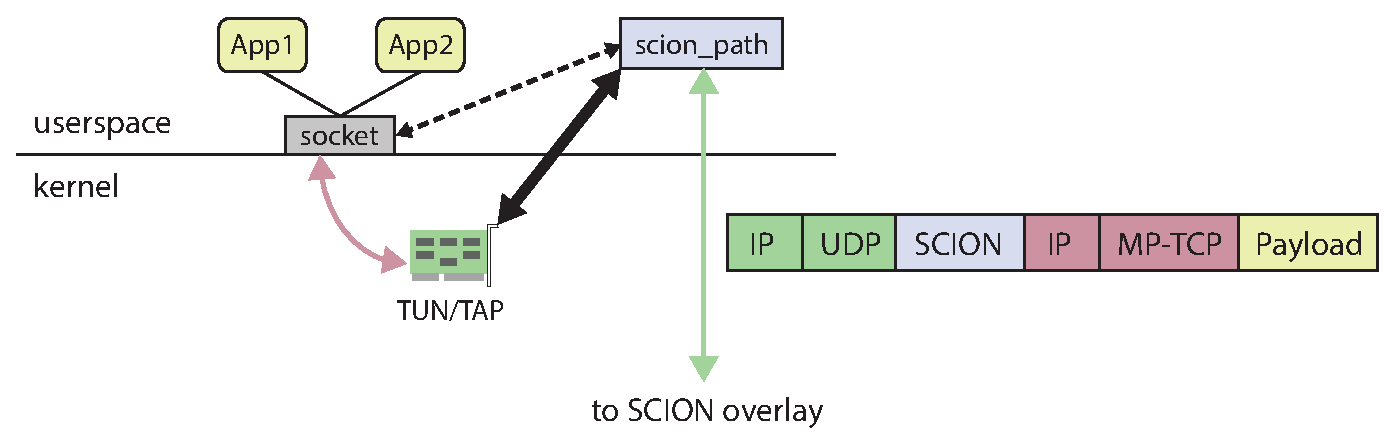
\includegraphics[width=1\columnwidth]{./fig/host2}
\end{minipage}
\caption{Host architecture.}\label{fig:host}
\end{figure}

\section{High-level architecture} \chris{outdated, this will change to the final SCION host architecture when it is decided}


Figure~\ref{fig:host} illustrates the architecture of a SCION host.
Normally, a SCION host has the following components.

\begin{itemize}
\item{\em SCION Socket} implements the SCION\_INET socket and provides the SCION socket API to allow user applications to communicate with each other with SCION packets.

\item{\em Name Resolution Client (NRC)} is a permanent user-space process serving all applications that resolves and caches domain names by sending out name resolution requests to Name Resolution Servers in local or remote ADs.

\item{\em Path store in user space} stores half-paths with the associated path metric information. % from PSes within the AD.

%\item{\em Path engine in kernel} contains end-to-end paths with associated information, which are computed according
%to the half-paths in Path engine.

\item{\em SCION layer in kernel} constructs complete SCION packets for applications, and forward the packets according to the routing paths stored in Path
table. Path table contains end-to-end paths with associated
information, which are computed according to the half-paths in Path
store.

\item{\em Multipath TCP module in kernel} allows user applications to use multiple TCP flows to the same destinations over different routing paths stored in path store.

\item{\em Path configuration daemon (PCD) in user space} allows system administrators
to configure path store upon startup, e.g., setting {\em preference
of neighbor ADs} and {\em the number of paths} used to deliver the
packets to the {\em ports} of the {\em destinations}. In the
meanwhile, PCD retrieves half-paths from the PSes within the AD
according to the configurations, and store them in the path store.
Note that, path store parameters are also used to configure
Multipath TCP (MP-TCP) parameters, e.g., the number of paths also
specify the number of subflows for each TCP session, which means
that users can also modify the parameter of MP-TCP to obtain better
application performance. These parameters can be set in application
using the ioctl() system call. Normally, the daemon will set default
values for applications, and system administrators can modify the
default configurations for these applications.
%    (default number of flows, etc) %stores path information.
\end{itemize}

%Figure with host architecture
%- Explain basic components
%  - Host application library
%  - SCION module in kernel
%  - Multipath TCP module in kernel
%  - Path table in kernel, contains half-paths with associated information
%  - Path engine in kernel, contains end-to-end paths with associated information
%  - Path configuration deamon in user space stores path information and
%    configures path table upon startup, configuration of Multipath TCP module
%    (default number of flows, etc)

\begin{figure}[ht]
\centering
\begin{minipage}{0.85\textwidth}
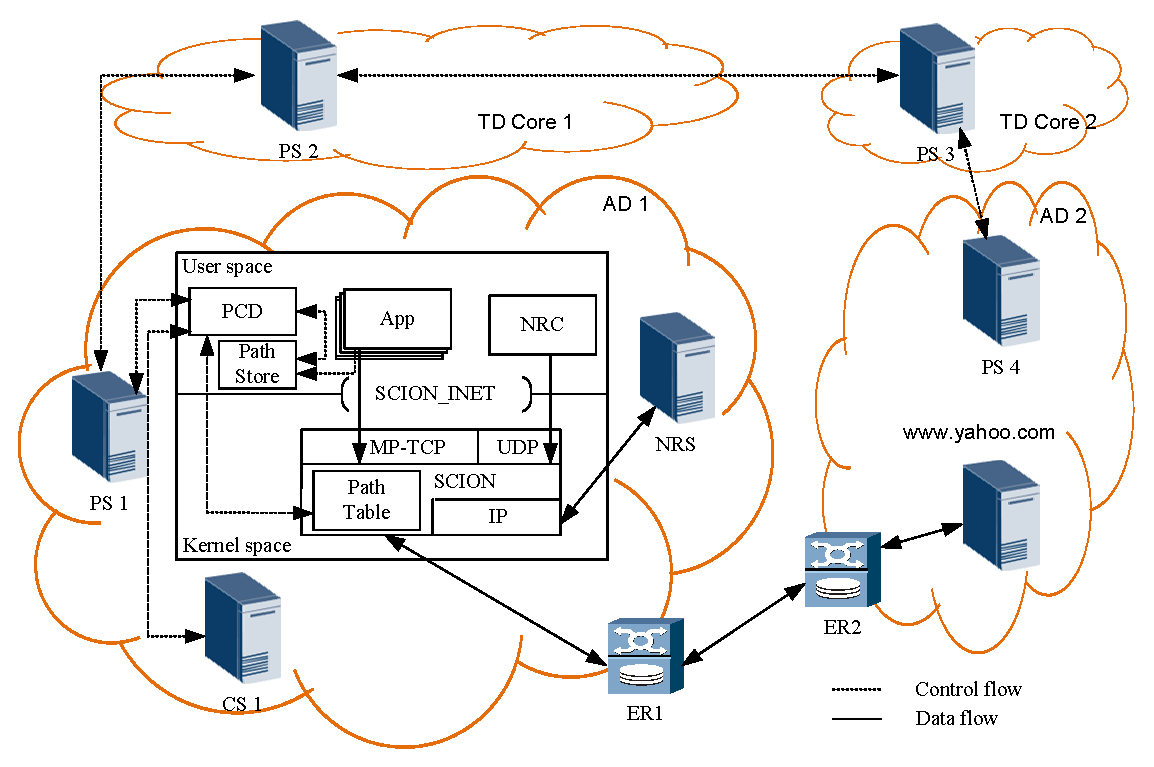
\includegraphics[width=1\columnwidth]{./fig/host.eps}
\end{minipage}
\caption{Host architecture.}\label{fig:host}
\end{figure}

%\begin{figure}[ht]
%\centering
%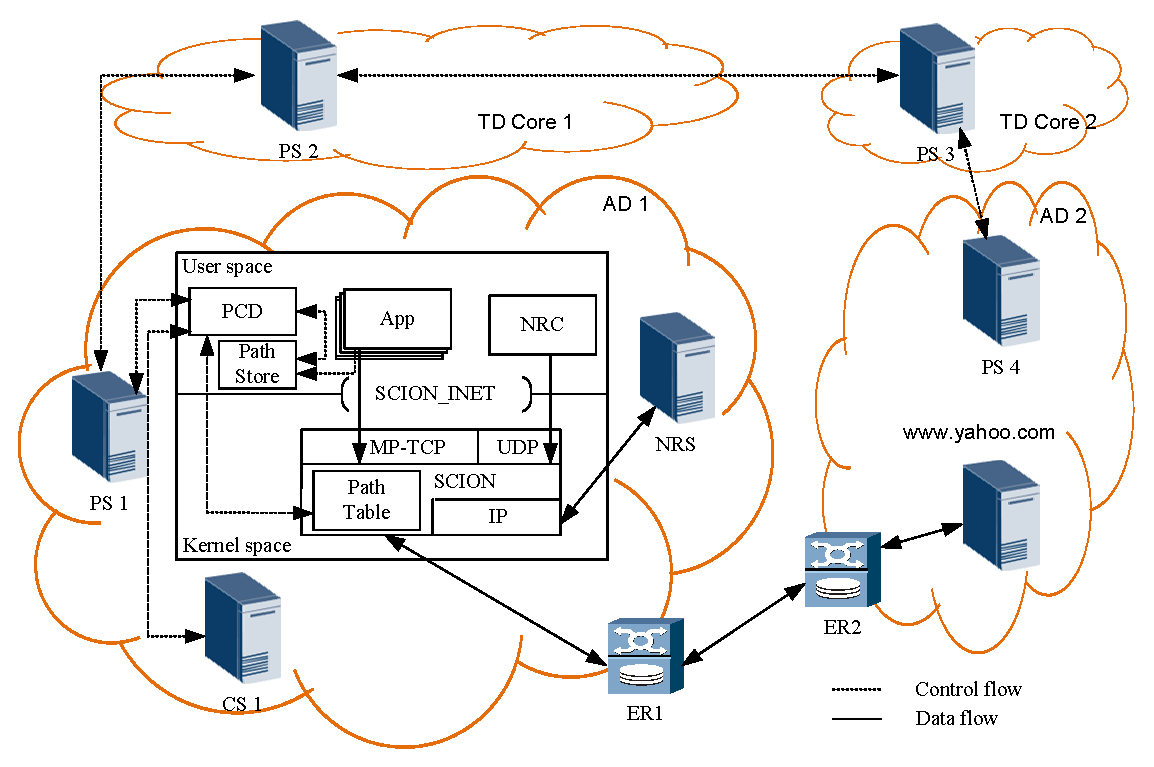
\includegraphics[width=.85\columnwidth]{./fig/host.eps}
%\caption{Host architecture.}\label{fig:host}
%\end{figure}

Each SCION host needs to obtain the correct information of different
servers, e.g., the address of PS, CS, and ER, before sending SCION
packets to the network. Such information is specified in the
topology file. Initially, only a CS address is configured in each
host, and then the host retrieves and loads the topology file from
the CS. After reading the topology file, the host regularly contacts
the CS to check for newer versions of the topology file. Normally,
an AD will have multiple CSes, PSes, and edge routers to obtain
fault tolerance to single CS failure. If any server will be taken
away, the new server will be setup before that.
%Since the
%topology file contains multiple CSes, the host can contact different
%CSes to update its topology file to obtain fault tolerance to single
%CS failure.
Also, the RoT file is initially installed in hosts. If
RoT file is not installed, the host can download it from CSes.

%Configuration of host:
%- Initially, only CS address has to be configured, from which topology file is loaded
%- Later, reading of topology file, contacting CS to check for newer
%  versions. Since topology file contains multiple CSs, we obtain fault tolerance
%  to single CS failure
%- RoT file is initially installed in host, if not, download from CS

\section{Example of host-to-host communication}

Now we use an example to illustrate how two end-to-end SCION hosts
can communicate with each other. We assume ISD Cores are operational
and that Name Resolution Server in each ISD Core resolves the
name-to-(local SCION address, AD) binding. In the example, we
suppose that the user, i.e., host in Figure~\ref{fig:host}, intends
to open a TCP connection to www.yahoo.com. Note that, if the host
bootstraps, it will contact the CS for the updated topology file and
then get the addresses of the PS and the ER. The procedure to  UDP
packets is similar, and we do not repeat here.

Applications can obtain name to AD/Address resolution via Name
Resolution Server (NRS) by the {\em getscionhostbyname()} function,
which is extended from the default function gethostbyname() and
implemented in host application library. With the function, host can
reach local NRS by using IP packets. The resolution results of
www.yahoo.com will be stored in the hostent struct. Later, we want
to use SCION anycast to reach NRS within the same domain.

Application opens SCION socket with destination address and AD as
parameters using the function as follows: {\em socket(SCION\_INET,
SOCK\_STREAM, 0))}, where SCION\_INET indicates that the application
wants to generate SCION packets and SOCK\_STREAM denotes that the
application uses TCP connection. After creating SCION the socket,
the ioctl() system call can be used to specify the parameter of the
socket, e.g., which paths within the AD will be preferred. Then, the
application uses the {\em connect()} function with the created
socket and the SCION address specified in the hostent struct as the
parameters to send TCP handshaking packets to the server. If the
socket is successfully connected, the host can read and write
packets via the socket so that it can communicate with the
destination server.

In a low level, all packets generated by the application will be
delivered from the TCP layers to the SCION layer in kernel to
construct complete SCION packets. In the SCION layer, path table
will be lookuped to obtain the correct routing paths for packet
delivery. If the paths are not cached in path table and there does
not exit any entry for the destinations in path store, PCD will
contact local PS to obtain correct paths to the destination. The
communication to local PS is same as communicating with NRS
discussed above. If the destination is in the remote AD, the PSes
will contact the PSes in the ISD core to obtain the paths. As shown
in Figure~\ref{fig:host}, www.yahoo.com is not within the same ISD.
The PSes forwards the path retrieval request to the PSes in ISD
core1, and the PS in ISD core1 will respond to the request with the
paths that are retrieved from ISD core2. Normally, PCD will retrieve
paths from the PS for different destinations and record them in path
store once the applications are installed. To allow applications and
system administrators can specify path selection preference, each
path in path store will be stored with more path quality
information, e.g., path bandwidth and delay.
%launched, and the
%destination addresses are recorded in PCD when the application are
%installed.
%PCD , the path store will retrieve the
%paths for the application and periodically contact update the paths.
Later, we will add APIs and command lines to enable configuring path
selection policies in path table by system administrators.

Path store will build end-to-end paths by joining up-paths and
down-paths that are retrieved from the PS according to routing
selection policies, and insert the result of end-to-end paths to
path table. The SCION layer lookups the path table and gets the
end-to-end paths to deliver the packet, and then construct the SCION
packet by putting the complete path information in the SCION header. %If the destination
%within the same AD, the SCION packet will be delivered to the
%destination according to the information in SCION header. Otherwise,
The packet will be sent to ER for further delivery. For example, as
shown in Figure~\ref{fig:host}, the packets to www.yahoo.com will be
sent to ER2, and then finally gets to the server.

To fully utilize the features of SCION, the future SCION\_INET
socket implementation can build end-to-end paths according to the
QoS parameter and routing policy parameters, which are configured by
application developers by using the ioctl() system call, or system
administrators by using path configuration daemon, based on the
local network performance, the application performance requirements,
and path selection preference. In the meanwhile, SCION can also
allow system administrators to directly specify entire end-to-end
paths for the applications that can be identified with the
destination addresses and the corresponding ports.
%\qi{Normally, applications cannot know the path
%information and user preference in each host so that they may not
%choose correct paths for users. Instead, users can easily use these
%information. So, I think it would be good to configure these stuffs
%in the path configuration daemon by users, e.g., according to the
%network performance and the user preference.}

%- later API: QoS parameters, routing policy parameters
%- even later API: entire end-to-end paths

%AD to path resolution via local Path Server (local PS) if destination AD
%information is not cached. Contacting local PS is done same as contacting NRS
%above. Add half-paths to path table
%- Maintain a default path table in the Kernel, but later, add API that enables
%  configuring path selection policies.
%- Define the path table structure that reflects path quality (e.g.,
%  bandwidth, delay, and so on)

%Build an end-to-end path by joining up-paths and down-paths from path table,
%insert end-to-end paths to path engine

%Create a SCION packet

%Send a packet using the SCION module, sent to ER in case destination is in
%different AD.

\section{Implementation Details}

\subsection{Overview: Implementation in Linux}

We implement the Path Store and PCD in the Linux user space (see
Figure~\ref{fig:host}. Other components are implemented in the
kernel space. We implement a SCION socket called the SCION\_INET
family to allow applications to create SCION packets, implement a
SCION layer in the networking stack, which lookups the path table
and constructs SCION packets, and a virtual network device, sciond,
which is used to transmitting and receiving SCION packets.
Figure~\ref{fig:kernel} illustrates the implementation of SCION
hosts in the kernel space. If an application create a SCION socket,
and the generated packets will be go through the TCP and the UDP
layers as normal. Before the packets get into the IP layer, the
packets will be hooked at the netfilter NF\_INET\_LOCAL\_OUT hook.
All packets labeled with SCION\_SOCKET family will be injected into
the SCION layer. The SCION layer will replace the IP headers with
the SCION header, and construct complete SCION packets and deliver
them to sciond. For the case of receiving packets, any SCION packets
getting to sciond will be delivered to sciond. In sciond, the SCION
headers will be replaced with IP headers, and the packets will go
through the legacy network and transport layers and be delivered the
applications.

\begin{figure}[ht]
\centering
\begin{minipage}{0.65\textwidth}
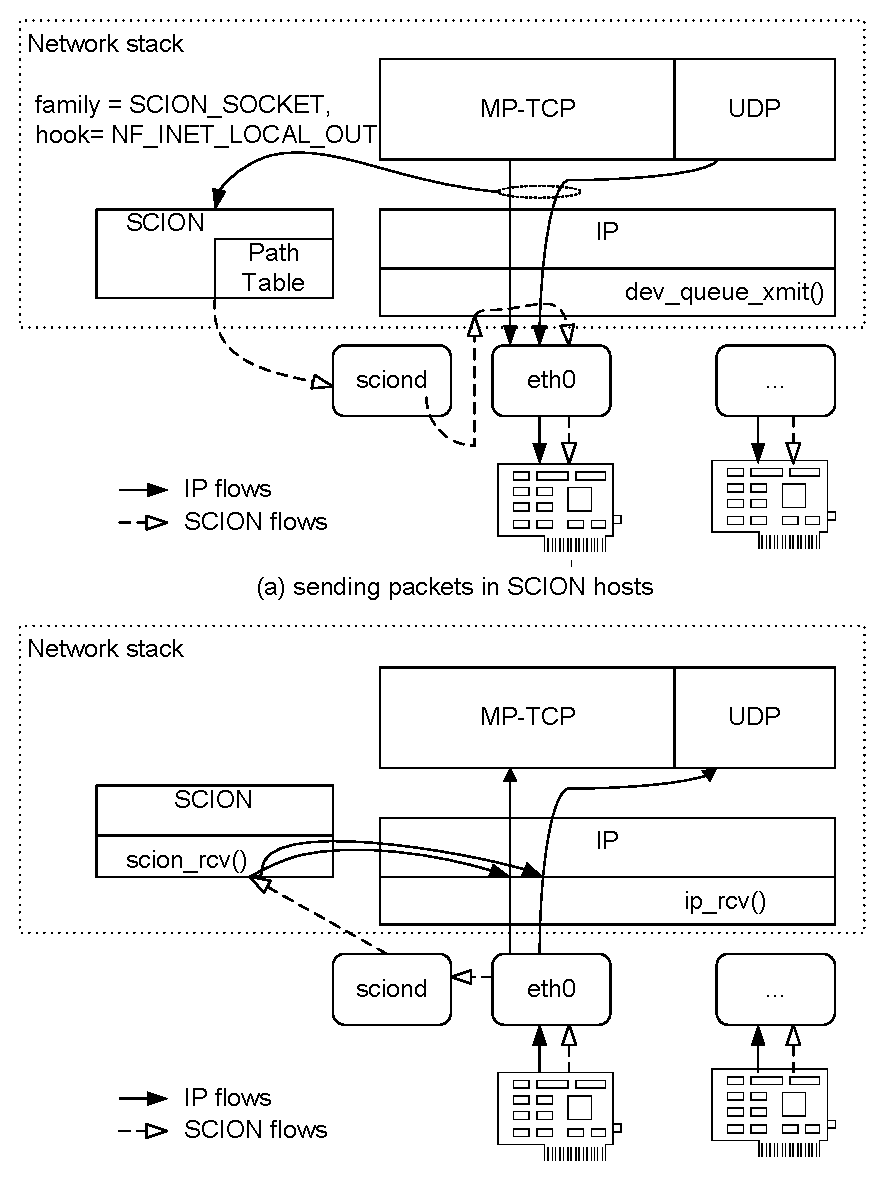
\includegraphics[width=1\columnwidth]{./fig/host_kernel.eps}
\end{minipage}
\caption{SCION implementation in Linux kernel.}\label{fig:kernel}
\end{figure}

The advantage of the implementation design is oblivious because we
cam enable SCION in the end host without any modification in
applications and the transport layer. Therefore, legacy applications
can easily use the SCION packets to communicate with the
destinations by configurations in PCD. In the meanwhile, the SCION
hosts can fully share the benefits of the existing mechanisms in the
current networking stack, e.g., we can directly use MP-TCP to enable
packet delivery over multipaths. Moreover, SCION hosts can achieve
much better performance with multipath packet delivery than the
traditional MP-TCP in the legacy hosts by enabling fine-grained path
selections according the path metric piggybacked in the path
announcements, i.e., beacons.

\subsection{Key Modules}

To fully implement SCION host architecture, SCION hosts have the
following blocks.

\begin{itemize}
\item{Implementation of the SCION\_INET Socket.}\ \ We will implement the following prot\_ops
structs and the related functions to enable the SCION socket API. We
only need to define a new family name and implement a scion\_ioctl
system call to allow application developers to specify path
selection policies in the applications, e.g., preferring paths
within the same ISD. Other functions are not changed as the
traditional inet\_stream\_ops and inet\_dgram\_ops structs,
respectively.

\begin{footnotesize}
\begin{lstlisting}[language=C]
 struct proto_ops scion_stream_ops = {
          .family         = SCION_INET,
          .owner          = THIS_MODULE,
          .release        = inet_release,
          .bind           = inet_bind,
          .connect        = inet_stream_connect,
          .socketpair     = sock_no_socketpair,
          .accept         = inet_accept,
          .getname        = inet_getname,
          .poll           = tcp_poll,
          .ioctl          = scion_ioctl,
          .listen         = inet_listen,
          .shutdown       = inet_shutdown,
          .setsockopt     = sock_common_setsockopt,
          .getsockopt     = sock_common_getsockopt,
          .sendmsg        = tcp_sendmsg,
          .recvmsg        = sock_common_recvmsg,
          .mmap           = sock_no_mmap,
          .sendpage       = tcp_sendpage,
          .splice_read    = tcp_splice_read,
 }
\end{lstlisting}

\begin{lstlisting}[language=C]
 struct proto_ops scion_dgram_ops = {
          .family         = SCION_INET,
          .owner          = THIS_MODULE,
          .release        = inet_release,
          .bind           = inet_bind,
          .connect        = inet_dgram_connect,
          .socketpair     = sock_no_socketpair,
          .accept         = inet_no_accept,
          .getname        = inet_getname,
          .poll           = udp_poll,
          .ioctl          = scion_ioctl,
          .listen         = sock_no_listen,
          .shutdown       = inet_shutdown,
          .setsockopt     = sock_common_setsockopt,
          .getsockopt     = sock_common_getsockopt,
          .sendmsg        = inet_sendmsg,
          .recvmsg        = sock_common_recvmsg,
          .mmap           = sock_no_mmap,
          .sendpage       = inet_sendpage,
 }
\end{lstlisting}
\end{footnotesize}

\item{Implementation of the SCION Layer and Virtual Device.}\ \
The SCION layer needs to lookup path table and deliver SCION packets
from and to the transport layer. Normally, we hook all packets from
the transport layer, and redirect the packets to the SCION layer if
the packet family specified in the sk\_buff struct is the
SCION\_INET family. The SCION layer lookups the path table to
retrieve the path information,
i.e., the Opaque information. %If the packets are for the remote
%destination,
and then replaces the IP header with the SCION headers. %will be
%inserted into the packets and the output device in the sk\_buff
%structure.
Then packets will be passed to the virtual device to finish packet
transmission. For the case of receiving packets, all SCION packets
will be delivered to the SCION packet handler, i.e., scion\_rcv(),
that fills in the IP headers in the sk\_buff struct, and then the
packets will delivered to the transport layer through the IP layer
for the purpose of enabling the normal packet processing procedure.
%If
%there does not exist any path entry in path table,
%tcp\_transmit\_skb() will directly pass the packets to
%ip\_queue\_xmit() for normal IP packet processing.

\item{Implementation of the Path Configuration Daemon.}\ \  Path PCD uses IP
packets to communicate with CSes to retrieve the topology file and
to contact PSes to request paths to the destinations. %In SCION
%hosts,
The retrieved up- and down-paths are stored in the path store (in
the user space). To avoid the delay of paths retrieval during
application startup, PCDs can pre-retrieve all half-paths for the
applications according to the system administrators' configurations.
%We can
%implement a Linux kernel module to create /proc nodes for all SCION
%related information. Then, all path configuration operations
PCD can directly create and modify path selection policies for
different destinations. We also allow PCD to directly modify the
end-to-end paths in the path table via the scion\_link socket that
is extended from the netlink socket.
%provided in path
%configuration daemon can be enabled by reading or modifying the
%corresponding node in the /proc filesystem. Later, we can add some
%system calls in the kernel so that the path configuration daemon can
%use the system calls to enable more fine-grained path configurations
%policies.
Moreover, by specifying the destination addresses and the port
number in PCD, legacy applications can also use SCION packets to
communicate with the corresponding destinations. Note that, path
selection policy configuration can be also enabled in applications
by using the ioctl() system call.
%, and the computed
%end-to-end paths in path table are maintained in Linux kernel

\item{Implementation of the Path Store.}\ \ It maintains up- and
down-paths learned from PSes, and compute the end-to-end paths
according to path configuration policies. The result end-to-end
paths will be inserted in the path table in the kernel space. %We
%implement a new socket called scion\_link that is extended from the
%netlink socket
The computed end-to-end paths in the path store will be updated to
the path table by using the scion\_link socket. The details of the
Path Store implementation and path selection policies will be
discussed in the next chapter.

\end{itemize}

%%% Local Variables:
%%% mode: latex
%%% TeX-master: "paper"
%%% End:
